 
\chapter{Spreadsheets}


\section{Libr\'{e} Office Calc}
\label{sec:calc}

\subsection{Introduction}

\subsubsection{tech}

Spreadsheets were one of the original ``killer apps'' when personal computers were first introduced.  Spreadsheets allow you to deal with tables of numbers and other data.  The standard convention is that the rows of a spreadsheet are indexed by numbers and the columns are indexed with letters.  If you need to go past 26 columns, use AA, AB, AC, {\em et cetera} for the next several columns.  It would be pretty unusual to need to have more than 702 columns but if you needed to, guess what comes after ZZ.

Suppose a businessman was in the completely legitimate business of making loans to people who are regarded as poor credit risks by conventional banks.  Of course, he'd want to keep track of the loan amounts and the recipients.  A spreadsheet is the perfect tool!

Here's a screen shot of how the data might be recorded:

\centerline{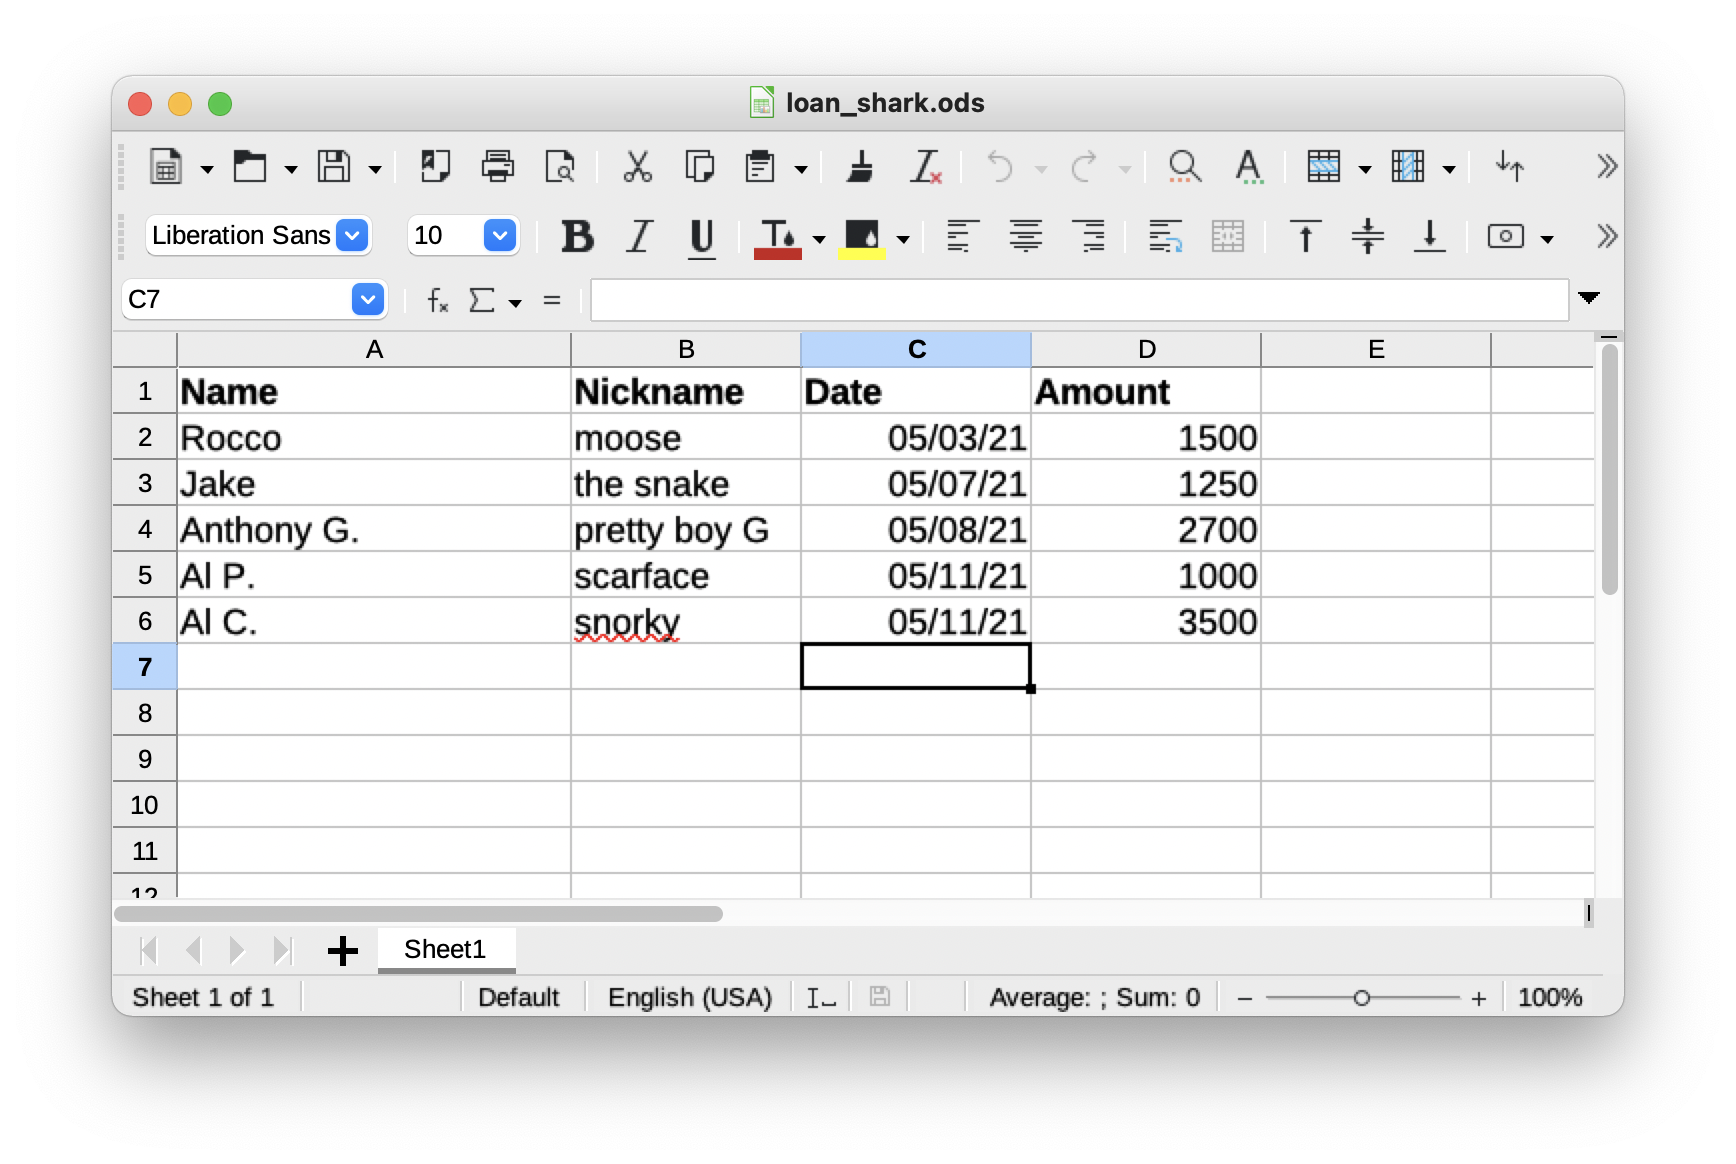
\includegraphics[scale=.5]{spread/loans.png}}

We're using the free/open-source Libr\'{e} Office spreadsheet in the above.  There are other choices (Excel on Windows and Numbers on Apple computers) but all of them work in a similar way and Libr\'{e} Office is free.  Spreadsheet files created by 
Libr\'{e} Office have a .ods suffix.  

The stuff that you enter into a cell in a spreadsheet fall into two main categories: a cell can contain data, or a cell can contain a calculated value.  To make a ``calculation''-type cell you have to put an equals sign up front.  When you're doing a calculation you can use the values that are in other cells by referring to them by column (letter) followed by row (number).  For example the \$3500 that Snorky borrowed is in cell D6.

\subsubsection{tasks}

Open the loan shark spreadsheet (the file is available on the book website) and make some additions -- columns for monthly interest rate, due date and the amount due.

Create a spreadsheet for keeping track of student grades in a math class. Use your favorite actors, sports stars, musicians (or whatever) as students, and just choose random numbers to put in as their grades. Create subtotals for homework, quizzes and exams, also a grand total with homework weighted $20\%$, quizzes weighted
$30\%$ and exams weighted $50\%$.



\subsection{Absolute and relative cell references}

\subsubsection{tech}

If you're going to be using the same calculation in a bunch of different places, you can just copy and paste the contents of one cell into another.  Get used to using the keyboard shortcuts Ctrl-C and Ctrl-V for copy and paste.  

When you copy and paste a formula, the spreadsheet intelligently changes the cell references in the formula.  The pasted formula refers to cells that are in the same positions {\em relative} to the spot we're pasting into.  

For example, if you type {\tt =B3 + C2}  into cell {\tt C3} you're telling the system to add the number just above and the number just to the left.  If you copy and paste that formula into cell {\tt K7} you'll find that the formula has become {\tt =J7+K6} because those cells are in the same relative positions.

This intelligent pasting {\em usually} does the right thing, but occasionally we really just want the thing to stay put!  If you want a cell reference to {\em not} change when you're cutting and pasting (this is known as an absolute reference) put dollars (\$) in front of both the letter and the number.  Very occasionally we want a sort of hybrid behavior -- we can put the dollar on one but not the other.  For instance, if in a formula we refer to a cell using \$A3  (with the dollar on the A but not in front of the 3) when we copy and paste the A will stay an A, but the 3 will change appropriately.  Some people call this making either the row or the column ``sticky.''  

\subsubsection{math}

In today's activity we'll be looking at two mathematical concepts: binomial coefficients and difference tables.

Binomial coefficients are sometimes called {\em choice counters}.  For example, given a set of 5 options how many ways can we select 3 of them?  This would be the binomial coefficient $\binom{5}{3}$ which is equal to 10.  To pronounce that symbol in English use the word ``choose,''  so the symbol above is read as ``five choose three.''  That notation for binomial coefficients can be a little confusing since many people assume the fraction bar just got left off!  So be careful, $\binom{5}{3} \; = \; 10$, but $\left( \frac{5}{3} \right) \; = \; 1.666\ldots$  so (obviously) these are different -- don't imagine fraction bars where they don't actually appear!

There is another notation for the same quantities using a capital letter $C$.  To indicate ``five choose three'' in this notation write $_5C_3$.

So why are these choice counters called ``binomial coefficients''?   It turns out these numbers also appear when taking powers of a {\em binomial} -- a polynomial with just two terms.  Try computing $(x+1)^0$, $(x+1)^1$, $(x+1)^2$ and $(x+1)^3$.  Really, only the last of those is at all difficult!  Anything to the $0$ power is just $1$, anything to the $1$ power is itself, and the $2$nd power just requires the FOIL rule!

Blaise Pascal -- a French mathematician who was one of the founders of the field of probability -- was probably the first to notice the pattern when you write these things next to one another.


\begin{tabular}{c}
	$1$ \\
	$x+1$ \\
	$x^2+2x+1$ \\
	$x^3 + 3x^2 + 3x+1$\\
\end{tabular}

The pattern becomes easier to deduce if you remove all the powers of $x$ (and the plus signs) and just concentrate on the coefficients.

\begin{tabular}{c}
	$1$ \\
	$1 \quad 1$ \\
	$1 \quad 2 \quad 1$ \\
	$1 \quad 3 \quad 3 \quad 1$\\
\end{tabular}

 Numbers on the outside of each row are always 1.  Numbers in the middle of a row are just the sum of the two things above them.
 
 The arrangement of binomial coefficients into this triangular array is called Pascal's triangle.  Here's the first 5 rows:
 
 \begin{tabular}{c}
 	$1$ \\
 	$1 \quad 1$ \\
 	$1 \quad 2 \quad 1$ \\
 	$1 \quad 3 \quad 3 \quad 1$\\
 	$1 \quad 4 \quad 6 \quad 4 \quad 1$\\
 	$1 \quad 5 \quad 10 \quad 10 \quad 5 \quad 1$\\
 \end{tabular}
 
 Difference tables come from a very common form of analyzing a sequence.
 
 Suppose we asked, ``What comes next?'' in the following sequence.
 
 \[ 4, \quad 7, \quad 10, \quad 13, \ldots \]
 
 You probably notice rather quickly that successive terms in the sequence differ by the same number.  A difference table is just a formalized way of making the same observation -- except that if the differences don't seem to have an obvious pattern we might continue on taking the differences of the differences!
 
 Here's an example.  Suppose you're given the following sequence of numbers.
 
 \[ 2 \quad 5 \quad 12 \quad 23 \quad 38 \quad \ldots \]
 
 A difference table looks like so:
 
 \begin{tabular}{ccccccccc}
 	2 &  & 5 & & 12 & & 23 & & 38 \\
 	   & 3 & & 7 & & 11 & & 15 
 \end{tabular}

SInce the differences don't exhibit an obvious pattern we continue on, obtaining

\begin{tabular}{ccccccccc}
	2 &  & 5 & & 12 & & 23 & & 38 \\
	& 3 & & 7 & & 11 & & 15 & \\
	& & 4 &  & 4  &  & 4 & & \\ 
\end{tabular}

It looks as though the bottom row -- which is known as the {\em second differences} is always 4.  Can you use that to predict what the next term in the sequence will be?

\subsubsection{tasks}

Write out the expanded form of $(x+1)^5$.

Create a table of the binomial coefficients $\binom{n}{k} = \frac{n!}{k!(n-k)!}$.

Revisit the grade spreadsheet from the previous section and insert a new row at the top.  Put the "weights" for homework, 
quizzes and exams into cells in this row.  (As the teacher you might want to experiment with different 
weighting schemes.) Are the final grades changed by much if we change the weights to 10, 
20 and 70 percent respectively?


Use a spreadsheet to do a finite differences analysis of the following sequence:

	  \[ 1 \quad 3 \quad 7 \quad 13 \quad 21 \ldots \]

Find the "back diagonals" for the sequences of squares, cubes, 4th powers etc.
(We care about back diagonals because you can use them to generate the entire sequence! (under the assumption that the bottom-most number is a constant) (sorry about all the parentheses)).

Maybe:
Given that the back diagonal for $x^n$ contains $s(n,k)*k!$ in the $k$th row, and the recursion for
the Stirling numbers.  Use a spreadsheet to create a table of the Stirling numbers.

\subsection{Builtin functions}

Tasks:

Returning to our gradebook example$\ldots$

Use the MIN function to "drop the lowest quiz."

Use functions to assign letter grades with $+$ and $-$ modifiers.
